\chapter{Estado del Arte\label{sec:estado_del_arte}}

\section{Gestión de redes\label{sec:gestion_redes}}
%%%%%%%%%%%%%%%%%%%%%%%%%%%%%%%%%%%%%%%%%%%%%%%%%%%%%%%%%%%%%%%%%%%%%%%%%%%%%%%%%%%%%%%%%%%%%%%%%%%%
El crecimiento de la complejidad de la estructura de las organizaciones en los últimos 40 años ha 
conllevado también aumento de la complejidad de sus redes de ordenadores. A medida que ampliamos y 
mejoramos nuestras redes, estas se vuelven más complejas y como resultado más difíciles de 
administrar. Si hace 40 años un administrador podría llevar a cabo su trabajo usando herramientas 
muy simples, con el tiempo estas han demostrado ser obsoletas e insuficientes y por este motivo se 
inició el desarrollo de las tecnologías de gestión de redes necesarias para igualar su nivel de 
sofisticación.

Durante su desarrollo, los investigadores, desarrolladores y usuarios del conjunto de protocolos 
DARPA/DoD TCP/IP han experimentado con un amplio conjunto de protocolos en diferentes entornos y 
configuraciones de red. La Internet empezó a crecer debido a la extendida disponibilidad de software
y hardware que comenzó a soportar este sistema. El crecimiento del el tamaño y el alcance de Internet
y cada vez su mayor uso en aplicaciones comerciales ha despertado en investigadores, desarrolladores y
fabricantes la necesidad de desarrollar un \textit{framework} común de gestión para los productos
TCP / IP.

Para satisfacer estas necesidades, diferentes esfuerzos empezaron a desarrollar conceptos de gestión
de redes que se pudieran aplicar a Internet y a sus tecnologías. Tres de estas tecnologías realizaron
suficientes progresos hacia finales de 1987 y quedo claro que la comunidad de desarrolladores tenía que
tomar algunas decisiones para no terminar trabajando un conjunto de herramientas incompatibles entre sí.
Estas tres tecnologías fueron el \textit{High-Level Entity Management System(HEMS)}, el \textit{Simple
Gateway Monitoring Protocol (SGMP)} y el \textit{Common Management Information Service/Protocol}.

Sin embargo, a corto plazo, la Internet necesitaba desesperadamente alguna herramienta que solucionase
los problemas de gestión asociados con su rápido crecimiento. Dado el estado actual de la implementación
de SGMP y su simplicidad, el consenso general fue que este protocolo debe evolucionar a una especificación
más completa para poder realizar su despliegue de forma extendida. Poco después, \textbf{\textit{Simple 
Network Management Protocol (SNMP) }} sustituyo el protocolo SGMP por su facilidad de uso y versatilidad.

A principios del siglo XXI quedó de manifiesto que a pesar de su objetivo original, SNMP no se usaba para
tareas de configuración sino como una herramienta de monitorización de redes. En Junio de 2002 la La Junta
de Arquitectura de Internet (Internet Architecture Board o IAB) y miembros clave de la comunidad \gls{IETF}
se reunieron para evaluar la situación. Los resultados de esas reuniones están documentados en el RFC 3535.
Principalmente, los operadores de red utilizaban principalmente \glspl{CLI} propietarias para configurar sus
dispositivos. Además, muchos fabricantes ni siquiera proporcionaban la opción de configurar sus dispositivos
mediante SNMP. Estas \gls{CLI} tenían algunas características que gustaban a los operadores de red,
principalmente que usaban protocolos basados en texto a diferencia de SMNP que usaba una codificación BER.
Aproximadamente al mismo tiempo, Juniper Neworks empezó a experimentar con sistemas de gestión basados en
\gls{XML}, hecho compartido con la \gls{IETF} que dio  lugar a la creación del Grupo de Trabajo NETCONF cuyo
principal objetivo fue la creación de un protocolo de configuración de redes que se ajustase a las necesidades
de los operadores de red y fabricantes de dispositivos. La primera versión del protocolo se publicó en el
\textit{RFC4741} en Diciembre de 2006 con varias extensiones publicadas en los años siguientes. Una versión
mejorada del protocolo fue publicada en el \textit{RFC6241} en Junio de 2011.

En 2015 Google desarrollo el protocolo \gls{gRPC} de baja latencia basado el \gls{HTTP}/2.0. A continuación 
se desarrolla también el protocolo \gls{gNMI} proporcionando características parecidas a Netconf pero 
mejorando algunos aspectos. En primer lugar \gls{gNMI} usa Protobuf para serialización de datos dando resultado 
a mensajes de tamaño más reducido comparado con \gls{XML}. También soporta de forma nativa el streaming 
bidireccional de información muy útil para telemetría mientras que NETCONF requiere usar las extensiones 
Yang PUSH. La última especificación de este protocolo es la versión 0.6.0 publicada el 30 de enero de 2018. 

\subsection{Simple Network Mangement Protocol\label{sec:SNMP}}
%%%%%%%%%%%%%%%%%%%%%%%%%%%%%%%%%%%%%%%%%%%%%%%%%%%%%%%%%%%%%%%%%%%%%%%%%%%%%%%%%%%%%%%%%%%%%%%%%%%%
\gls{SNMP} es un protocolo de capa de aplicación usado para la recolección y organización de
información de los dispositivos gestionados y la modificación de dicha información con el fin de 
modificar el comportamiento de dichos dispositivos. Entre los dispositivos que soportan SNMP 
encontramos módems, router, switches, servidores, estaciones de trabajo, etc.

La base de \gls{SNMP} es un simple conjunto de operaciones que permite a los administradores cambiar el
estado de dispositivos SNMP. Por ejemplo, se puede usar \gls{SNMP} para apagar una interfaz de un router o
comprobar la velocidad a la que una interfaz Ethernet está operando. 

\subsubsection{Gestores y Agentes}

En el mundo \gls{SNMP} existen dos tipos de entidades: gestores (\gls{SNMP} Managers) y agentes. 

%%%%%%%%%%%%%%%%%%%%%%%%%%%%%%%%%%%%%%%%%%%%%%%%%%%%%%%%%%%%%%%%%%%%%%%%%%%%%%%%%%%%%%%%%%%%%%%%%%%%
Un \textbf{SNMP Manager} también llamado Sistema de Gestión de Red (Network Management System o NMS)
es una entidad responsable de la comunicación con los agentes SNMP disponible en la red. Típicamente
es un servidor que ejecuta uno o varios sistemas de gestión de red. Sus principales tareas son:

\begin{itemize}
    \item Consultar a los agentes
    \item Obtener las respuestas enviadas por los agentes
    \item Establecer o cambiar valores de variables en los agentes
    \item Recibir notificaciones eventos de los agentes de forma asíncrona
\end{itemize}

Los agentes SNMP con programas que recolectan información local de los dispositivos en los que están
instalador y la hacen disponible para los SNMP Managers. Las funciones de un agente SNMP son las
siguientes:

\begin{itemize}
    \item Recolectar información acerca de su entorno local
    \item Almacenar y devolver la información definida en sus bases de datos.
    \item Enviar señales a los gestores cuando ocurre un evento
    \item Actuar como un proxy para los nodos no gestionables mediante SNMP
\end{itemize}

En la Figura \ref{fig:diagrama_comunicaciones_snmp} podemos observar como se organizan estas dos
entidades. 

\begin{figure}[ht]
    \centering
    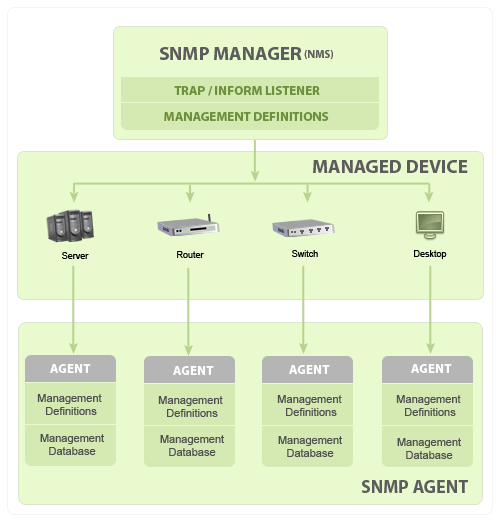
\includegraphics[width=10cm]{graphics/snmp-components}
    \caption{Diagrama básico de comunicaciones SNMP}
    \label{fig:diagrama_comunicaciones_snmp}
\end{figure}

%%%%%%%%%%%%%%%%%%%%%%%%%%%%%%%%%%%%%%%%%%%%%%%%%%%%%%%%%%%%%%%%%%%%%%%%%%%%%%%%%%%%%%%%%%%%%%%%%%%%
\subsubsection{\gls{MIB}}
La Base de Información Gestionada (\gls{MIB}) es un tipo de base de datos que contiene información
jerárquica, con estructura de árbol, de los parámetros gestionables de cada dispositivo SNMP. La
jerarquía MIB se organiza en distintos niveles que se asignan a distintas organizaciones. Los 
primeros niveles están asignados a organizaciones de normalización (ISO, CCITT, etc) mientras que 
los niveles más bajos están asignadas a organizaciones asociadas. En la Figura \ref{fig:mib_tree} 
se puede observas esta forma de organización.


Existe un gran número de MIBs definidos por organizaciones como la \gls{IETF} así como entidades
privadas y fabricantes. La base de datos más común para la gestión de equipos en Internet es la base
MIB-II definida en el \textit{RFC1213} y ampliada con la aparición de las versiones 2 y 3 de SNMP. 
Este MIB es muy importante porque es obligatorio para todos los agentes SNMP de internet y contiene
información acerca del sistema, interfaces así como aspectos de IP (incluidas las tablas de
enrutamiento).


Todos los objetos tienen un identificador único denominado OID que permiten la identificación numérica
de cualquier nodo. Por ejemplo, sirviéndonos de la Figura \ref{fig:mib_tree} podemos ver que el del
objeto \textit{iso.org.dod.internet.mgmt.mib-2.system.sysDescr} tiene el OID 1.3.6.1.2.1.1.1.

\begin{figure}[ht]
    \centering
    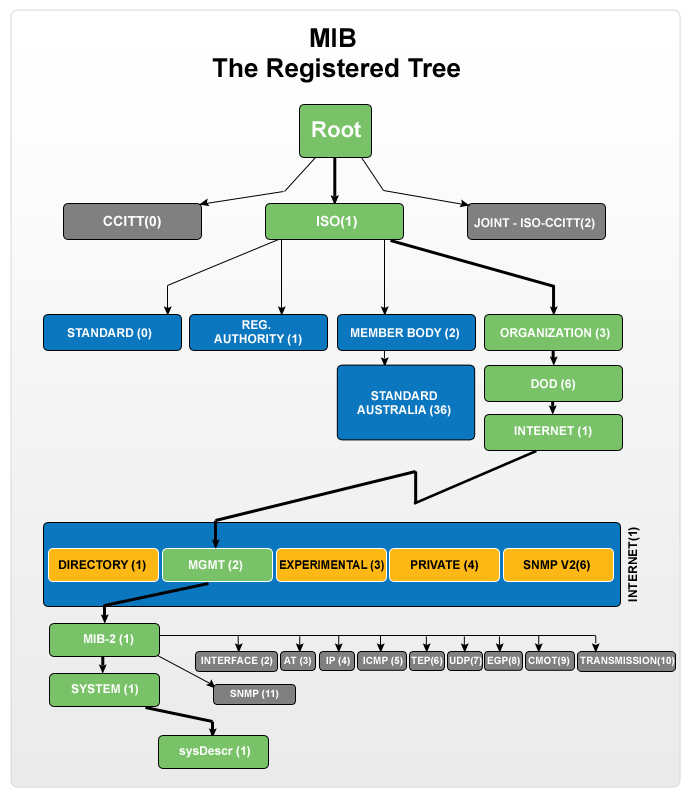
\includegraphics[width=10cm]{graphics/mib-oid-tree}
    \caption{Árbol MIB (parcial)}
    \label{fig:mib_tree}
\end{figure}

%%%%%%%%%%%%%%%%%%%%%%%%%%%%%%%%%%%%%%%%%%%%%%%%%%%%%%%%%%%%%%%%%%%%%%%%%%%%%%%%%%%%%%%%%%%%%%%%%%%%
\subsubsection{Operaciones básicas de SNMP}

Las operaciones que pueden realizar dentro del protocolo SNMP son las siguientes
\cite{mauro2005essential}:

\begin{itemize}
    \item GET: La operación GET es una petición enviada por un gestor a un agente para obtener uno o
    más valores del agente. Figura \ref{fig:snmp_get}
    \item GET NEXT: Esta operación es similar a GET. La principal diferencia es que GET NEXT obtiene
    el valor del siguiente OID del árbol MIB.
    \item GET BULK (SNMPv2 y v3): Operación usada para obtener grandes volúmenes de datos desde tablas
    MIB grandes.Figura \ref{fig:snmp_bulk}
    \item SET: Esta operación es usada por los gestores para modificar o asignar un valor dentro de un
    agente.Figura \ref{fig:snmp_set}
    \item TRAPS: Los TRAPS son señales enviadas por los agentes para notificar a los gestores de algún
    evento.Figura \ref{fig:snmp_trap}
    \item INFORM: similar a una TRAP, pero a diferencia de este INFORM incluye la confirmación por
    parte del gestor \gls{SNMP} de la recepción del mensaje
    \item RESPONSE: este es el comando usado para devolver valores a los gestores SNMP.
\end{itemize}

\begin{figure}
    \centering
    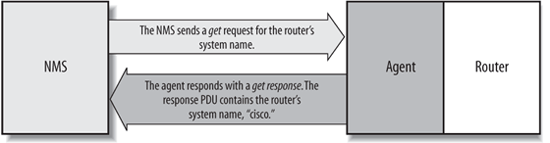
\includegraphics[width=.5\linewidth]{graphics/snmp_get}
    \caption{SNMP Get Sequence}
    \label{fig:snmp_get}
\end{figure}

\begin{figure}
    \centering
    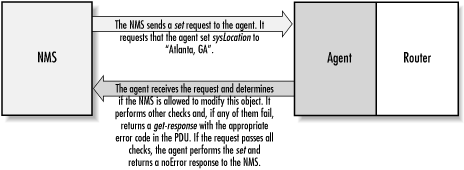
\includegraphics[width=.5\linewidth]{graphics/snmp_set}
    \caption{SNMP Set Sequence}
    \label{fig:snmp_set}
\end{figure}

\begin{figure}
    \centering
    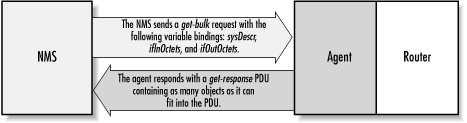
\includegraphics[width=.5\linewidth]{graphics/snmp_get_bulk}
    \caption{SNMP Get Bulk Sequence}
    \label{fig:snmp_bulk}
\end{figure}

\begin{figure}
    \centering
    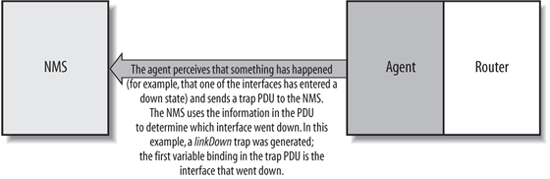
\includegraphics[width=.5\linewidth]{graphics/snmp_trap}
    \caption{SNMP Trap Sequence}
    \label{fig:snmp_trap}
\end{figure}

\subsection{Network Configuration Protocol\label{sec:NETCONF}}

\subsection{Google Network Management Interface\label{sec:gNMI}}

\section{Yang Data Model}

\subsection{Introducción al modelado YANG}

\subsection{OpenConfig modelos}

\section{Telemetría}

\subsection{Framework}

Resumen de
https://tools.ietf.org/id/draft-opsawg-ntf-00.html

\subsection{Network Configuration Notifications\label{sec:NETCONFNot}}

https://tools.ietf.org/html/rfc5277

\subsection{YANG Push Notifications\label{sec:YANGNot}}

https://datatracker.ietf.org/doc/rfc8641/
https://tools.ietf.org/id/draft-ietf-netconf-notification-capabilities-05.html
